%%%%%%%%%%%%%%%%%%%%%%%%%%%%%%%%%%%%%%%%%%%%%%%%%%%%%%%%%%%%%%%%%%%%
%% AI-Based Cancer Detection System Presentation
%% Using the fibeamer theme
%%%%%%%%%%%%%%%%%%%%%%%%%%%%%%%%%%%%%%%%%%%%%%%%%%%%%%%%%%%%%%%%%%%%

\documentclass{beamer}
\usetheme[faculty=ped]{fibeamer}

\usepackage[utf8]{inputenc}
\usepackage{graphicx}
\usepackage{booktabs}
\usepackage{tikz}
\usepackage{amsmath}

\title{AI-Based Cancer Detection System}
\subtitle{Early Detection using Machine Learning}
\author{Aditya}
\date{\today}

\begin{document}

\frame[c]{\maketitle}

%------------------------------------------------

\begin{frame}{The Problem}
\begin{itemize}
\item Cancer diagnosis often occurs too late
\item Manual analysis is time-consuming
\item Early detection can significantly improve survival rates
\end{itemize}
\end{frame}

%------------------------------------------------

\begin{frame}{Project Objective}
\begin{itemize}
\item Develop an AI-powered cancer detection system
\item Predict whether a tumor is benign or malignant
\item Assist healthcare professionals using machine learning
\end{itemize}
\end{frame}

%------------------------------------------------

\begin{frame}{Dataset}
\begin{itemize}
\item Breast Cancer Dataset
\item Features include:
\begin{itemize}
\item Radius
\item Texture
\item Smoothness
\item Compactness
\end{itemize}
\item Target Classes:
\begin{itemize}
\item Benign
\item Malignant
\end{itemize}
\end{itemize}
\end{frame}

%------------------------------------------------

\begin{frame}{Data Preprocessing}
\begin{itemize}
\item Data Cleaning
\item Feature Scaling using StandardScaler
\item Train-Test Split
\item Label Encoding
\end{itemize}
\end{frame}

%------------------------------------------------

\begin{frame}{Machine Learning Model}
\begin{itemize}
\item Random Forest Classifier
\item Logistic Regression
\item Model trained using sklearn
\end{itemize}

\vspace{0.5cm}

\textbf{Why Random Forest?}
\begin{itemize}
\item High accuracy
\item Handles complex patterns
\item Reduces overfitting
\end{itemize}
\end{frame}

%------------------------------------------------

\begin{frame}{System Workflow}
\centering

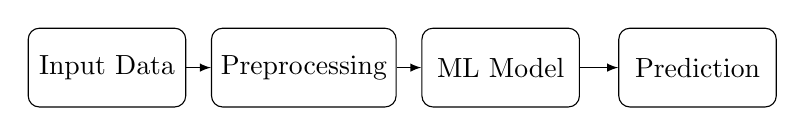
\begin{tikzpicture}[node distance=2.5cm, auto]
\tikzstyle{block} = [draw, rectangle, rounded corners, minimum height=1cm, minimum width=2cm, text centered]
\tikzstyle{line} = [draw, -latex]

\node [block] (input) {Input Data};
\node [block, right of=input] (pre) {Preprocessing};
\node [block, right of=pre] (model) {ML Model};
\node [block, right of=model] (output) {Prediction};

\path [line] (input) -- (pre);
\path [line] (pre) -- (model);
\path [line] (model) -- (output);

\end{tikzpicture}

\vspace{0.7cm}

Prediction Output:
\begin{itemize}
\item Benign
\item Malignant
\end{itemize}

\end{frame}

%------------------------------------------------

\begin{frame}{Results}

\begin{table}
\centering
\begin{tabular}{lc}
\toprule
Metric & Value \\
\midrule
Accuracy & 95\% \\
Precision & 94\% \\
Recall & 96\% \\
F1-Score & 95\% \\
\bottomrule
\end{tabular}
\end{table}

\vspace{0.5cm}

\textbf{Outcome:}
The model achieved high accuracy in cancer classification.

\end{frame}

%------------------------------------------------

\begin{frame}{Model Prediction Example}

\begin{itemize}
\item Input patient data processed
\item Model generated prediction
\item Output:
\begin{itemize}
\item Benign
\item Confidence Score: 92\%
\end{itemize}
\end{itemize}

\end{frame}

%------------------------------------------------

\begin{frame}{Challenges}
\begin{itemize}
\item Limited medical datasets
\item Risk of overfitting
\item Feature selection complexity
\item Data imbalance issues
\end{itemize}
\end{frame}

%------------------------------------------------

\begin{frame}{Future Scope}
\begin{itemize}
\item Deep Learning Integration
\item Real-time hospital deployment
\item Mobile healthcare applications
\item Multi-cancer detection system
\end{itemize}
\end{frame}

%------------------------------------------------

\begin{frame}{Conclusion}
\begin{itemize}
\item AI improves cancer diagnosis speed
\item Machine learning assists medical professionals
\item Early detection can save lives
\end{itemize}

\vspace{0.5cm}

\centering
\Huge Thank You
\end{frame}

\end{document}
